\chapter{Grundlagen}

In diesem Kapitel wird das Wissen vermittelt, welches benötigt wird um zu Verstehen, wie \acp{NNUE} im Rahmen von Schachcomputern funktionieren. Zuerst wird die Evaluation, wie sie in herkömmlichen Schachcomputern funktioniert erklärt, auch \ac{HCE} genannt. Weiterhin werden die grundlegenden Bestandteile, die für überwacht lernende \acp{FNN} von Bedeutung sind, eingegangen. Außerdem wird erläutert was \ac{SIMD} ist und wie diese Vektoroperationen in C/C++ verwendet werden können. Zuletzt wird die grundlegende Funktionsweise von \acp{NNUE} vermittelt, die auf den davor gelegten Grundsteinen aufbaut.

\section{Hand-crafted Evaluation}
\label{chap:HCE}

Es ist wichtig zu wissen wie die \ac{HCE} eines Schachcomputers funktioniert, da sie nicht nur die Variante die in jedem starken Schachcomputer vor 2017 eingesetzt wurde, sondern auch heute noch in Kombination mit \ac{NNUE} eingesetzt wird. Bei \ac{NNUE} Schachcomputern wird sie oft in Kombination mit der \ac{NN} evaluation genutzt, weil sie besser in extremen Stellungen funktioniert. Besitzt beispielsweise Weiß in einer Position eine Dame mehr, muss nicht die teurere Berechnung des \acp{NNUE} durchgeführt werden, um zu entscheiden, dass Weiß im Vorteil ist.

Die \ac{HCE} einer Schachposition ist eine heuristische Methode der Position einen numerischen Wert zuzuordnen. Vor der Verbreitung von \acp{NN}, war \ac{HCE} die einzige Form der Positions-Evaluation. Gäbe es unendliche Ressourcen könnten aus jeder Position alle mögliche Zugfolgen per Brute-Force bestimmen und der Positionen einer der drei Werte: -1 (Verlust), 0 (remis), 1 (Gewinn) geben. In der Realität ist es nicht möglich den exakten Wert der Stellung zu kennen, deshalb wird in der \ac{HCE} versucht anhand von Menschen festgelegten Kriterien einen Wert der Position zuzuordnen. Die so gewonnene Bewertung wird in der Zugsuche verwendet, um den besten Zug, abhängig von den per Hand gewählten Kriterien, zu finden. Die Evaluation wird aus Sicht der Seite, die gerade am Zug ist angegeben. Das ist wichtig für den verwendeten Suchalgorithmus (Alpha-Beta-Suche) \cite{Slagle1969}.

Die \ac{HCE} eines Schachcomputers ähnelt in einigen Aspekten mehr eine Philosophie als eine Funktion. Schach ist ein Spiel, das es seit über 1000 Jahren gibt. In dieser Zeit haben Menschen regeln überlegt, um besser Schach zu spielen. All diese Regeln in die Evaluationsfunktion zu integrieren, ist nicht ratsam. Es ist ein Abwägen zwischen Wissen und Geschwindigkeit. Je mehr regeln dem Computer geben werden, umso weniger weit kann er Vorausschauen.

Wenn ein Mensch Schach spielen lernt, ist der Wert der Figuren eines der ersten Erkenntnisse. Das ist ebenfalls der wichtigste Faktor für einen Schachcomputer \cite{Levy1988}. Die Angabe der Materialwertung wird bei Computern als Centipawn angegeben, um so mehr Spielraum für feingranulare Faktoren zu lassen. Figuren werden ebenfalls anhand ihrer Position bewertet. Dafür gibt es sogenannte Piece Square Tables, die jeder Figur abhängig von ihrer Position einen Wert zuordnen. Beispielsweise ist ein Springer am Rand des Brettes deutlich weniger Wert als einer im Zentrum, auch bekannt als \enquote{ein Springer am Rand bringt Kummer und Schand}. Weitere nennenswerte Aspekte der \ac{HCE} sind

% weitere evlauations aspekte

% erklären warum verschiedene Spielphasen eine rolle spielen

% vl noch was zu NNs

\section{Neuronale Netze}

\begin{figure}
  \centering
  % inspired by: https://tex.stackexchange.com/questions/153957/drawing-neural-network-with-tikz
  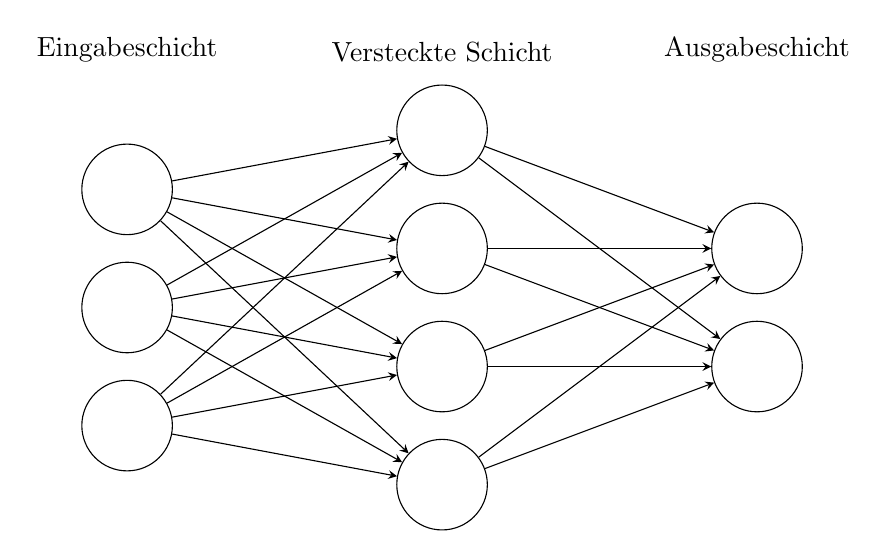
\begin{tikzpicture}[x=2cm, y=1.5cm, >=stealth]
    \tikzstyle{neuron}=[draw,shape=circle,minimum size=1.15cm]
    % draw nerons
    \foreach \m/\l [count=\y] in {1,2,3}
    \node [neuron] (input-\m) at (0,2-\y) {};

    \foreach \m [count=\y] in {1,2,3,4}
    \node [neuron] (hidden-\m) at (2,2.5-\y) {};

    \foreach \m [count=\y] in {1,2}
    \node [neuron] (output-\m) at (4,1.5-\y) {};
    % draw lines  
    \foreach \i in {1,2,3}
    \foreach \j in {1,2,3,4}
    \draw [->] (input-\i) -- (hidden-\j);

    \foreach \i in {1,2,3,4}
    \foreach \j in {1,2}
    \draw [->] (hidden-\i) -- (output-\j);

    \foreach \l [count=\x from 0] in {Eingabeschicht, Versteckte Schicht, Ausgabeschicht}
    \node [align=center, above] at (\x*2,2) {\l};
  \end{tikzpicture}
  \caption{Ein einfaches \acl{NN}}
  \label{fig:beispiel-nn}
\end{figure}

\Acp{KNN} oder einfach \acp{NN} genannt, sind Computer Systeme, die dem biologischen Vorbild des Gehirns nachempfunden sind. Analog zu seinem biologischen Vorbild besteht ein \ac{NN} aus Neuronen die miteinander Vernetzt sind. Jedes Neuron reagiert auf eingehende Signal mit einer bestimmten Reaktion. Diese Reaktion kann sich durch neu gewonnene Erfahrungen anpassen, das ermöglicht es zu lernen und zukünftig besser zu reagieren.

% erklären wie der generelle aufbau ist
In Abbildung \autoref{fig:beispiel-nn} ist ein einfaches \acl{NN} zu sehen. Es besteht aus drei Schichten. Die erste Schicht, die Eingabeschicht, nimmt Eingabedaten entgegen. Eingabedaten können ganz unterschiedliche daten Repräsentieren, ist der Eingabedatensatz beispielsweise ein 100×100 Schwarzweiß-Bild, ist eine Möglichkeit die Eingaben darzustellen. Die Eingabeschicht besteht dann aus 1000 Neuronen die pro Neuron den Zustand eines Pixels (0 = weiß, 1 = Schwarz) des Bildes gefüttert bekommen. Die zweite Schicht heißt versteckte Schicht, weil von außen nur die Eingabedaten und das Ergebnis sichtbar ist. Sie empfängt die Informationen der Eingabeschicht, gewichtet sie und gibt sie an der Ausgabeschicht weiter. Die versteckte Schicht kann aus mehreren Schichten bestehen. Ein \ac{NN} mit mehreren versteckten Schichten heißt \ac{DNN}. Die letzte Sicht, die Ausgabeschicht, spiegelt das Ergebnis des \acp{NN} dar. Ein Netz, das versucht Bilder zwischen Hunden und Katzen zu unterscheiden kann zwei Ausgabeneuronen enthalten, eins für die Wahrscheinlichkeit das auf dem gegebenen Bild ein Hund ist und eins für die Wahrscheinlichkeit das es eine Katze ist. Ein \ac{NN} kann auch nur ein Ausgabeneuron besitzen, wie \zb{} bei der Evaluation einer Schachposition nötig ist. Die Verbindungen der einzelnen Neuronen stellen deren Zusammenhang dar. Wie stark dieser Abhängigkeit ist, wird durch Gewichte definiert \cite[S. 2--7]{krawczak2013multilayer}.
% auswahl der Input daten spalten gibt an wieviele input neuronen es gibt, die anzal der hidden neuronen ist "egal" je mehr -> desto besser kann das neuronale netz lernen kinda, output neuronen gibt die anzahl der klassifikationen an, kann auch nur eins sein (regession)

Es gibt verschiedene Modelle \aclp{NN}, für diese Thesis sind lediglich \acp{FNN} relevant. \acp{FNN} basieren auf dem von \citeauthor{rosenblatt1958perceptron} \cite{rosenblatt1958perceptron} beschriebenen mehrlagigen Perzeptron. Das \ac{FNN} zeichnet sich durch seinen Zyklen freien Aufbau aus. Der Datenfluss führt immer von der Eingabeschicht zu Ausgabeschicht. Das \ac{FNN} gilt als die einfachste Netzwerkarchitektur \cite{Schmidhuber2015}.

In der Praxis, so auch in dieser Arbeit, werden für die Entwicklung neuronaler Netze Frameworks verwendet. Sie abstrahieren große Teile der Komplexität. Trotzdem ist es wichtig ihre Funktionsweise zu kennen, um Entscheidungen zu treffen und Probleme zu beheben. In den folgenden Unterabschnitten wird Grundlegend auf die Einzelteile neuronaler Netze eingegangen. Erst wird das Neuron beschrieben und wie sich seine Aktivität berechnen lässt. Das Unterkapitel Backpropagation beschreibt, wie \acp{NN} lernen können.

\subsection{Das Neuron}

\begin{figure}
  \centering
  % inspired by: https://davidstutz.de/illustrating-convolutional-neural-networks-in-latex-with-tikz/
  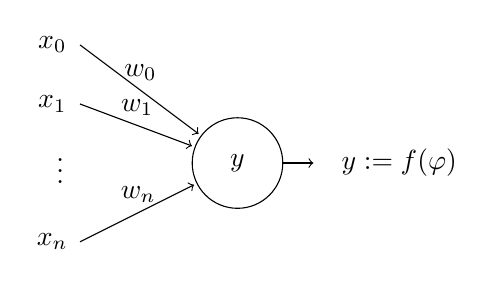
\begin{tikzpicture}[shorten >=1pt,->]
    \tikzstyle{unit}=[draw,shape=circle,minimum size=1.15cm]

    \node[unit](p) at (2,1){$y$};
    \node(dots) at (-0.25,1){\vdots};

    \draw (0,2.5) node[xshift=-10]{$x_0$} -- node [midway,above] {$w_{0}$} (p);
    \draw (0,1.75) node[xshift=-10]{$x_1$} -- node [midway,above] {$w_{1}$} (p);
    \draw (0,0) node[xshift=-10]{$x_n$} -- node [midway,above] {$w_{n}$} (p);
    \draw (p) -- (3,1) node[xshift=30]{$y := f(\varphi)$};
  \end{tikzpicture}
  \caption{Ein einzelnes Neuron mit seinen eingabe- und Ausgabekomponenten}
  \label{fig:neuron}
\end{figure}

% neuronen wie sie im nerfen systems eines menschen vorhanden sind
Das Neuron ist der elementare Bestandteil eines \acp{NN}. Es wurde \citeyear{McCulloch1943} von \citeauthor{McCulloch1943} \cite{McCulloch1943} eingeführt. Neuronen sind in einem \ac{NN} mit anderen Neuronen verbunden und bilden so beliebig komplexe Funktionen ab. In \autoref{fig:neuron} ist ein einzelnes Neuron zu sehen. Die Eingänge $x_{0}$ bis $x_{n}$, werden mit den Gewichten $w_{0}$ bis $w_{n}$ multipliziert und aufsummiert und mit der Aktivierungsfunktion $f(\varphi)$ wird die Ausgabe des Neurons. Für gewöhnlich ist immer $x_{0}=1$, was ihn zu dem Bias des Neurons mit $w_{0}=b$ macht. Das bedeutet, dass es nur $n$ tatsächliche Eingabewerte gibt: von $x_{1}$ bis $x_{n}$. Konkret lässt sich die Aktivität eines Neurons mit der \autoref{equation:NeuronActivation} und die Ausgabe $y$ mit \autoref{equation:NeuronOutput} bestimmen:

\begin{equation}
  f(\varphi) = \varphi(\sum_{i=0}^{n}w_{i}x_{i})
  \label{equation:NeuronActivation}
\end{equation}

\begin{equation}
  y = f(\varphi)
  \label{equation:NeuronOutput}
\end{equation}

\begin{figure}
  \centering
  \begin{subfigure}{.5\textwidth}
    \centering
    \resizebox{.9\textwidth}{!}{%
      \begin{tikzpicture}[declare function={sigma(\x)=1/(1+exp(-\x));}]
        \begin{axis}%
          [
            grid=none,
            xmin=-6,
            xmax=6,
            axis x line=bottom,
            ytick={0,.5,1},
            ymax=1,
            axis y line=middle,
            samples=100,
            domain=-6:6,
            legend style={at={(1,0.9)}}
          ]
          \addplot[blue,mark=none]   (x,{sigma(x)});
        \end{axis}
      \end{tikzpicture}
    }
    \caption{Standardsigmoide Aktivierungsfunktion}
    \label{fig:sigmoid}
  \end{subfigure}%
  \begin{subfigure}{.5\textwidth}
    \centering
    \resizebox{.9\textwidth}{!}{%
      \begin{tikzpicture}[declare function={relu(\x)=max(0,\x);}]
        \begin{axis}%
          [
            grid=none,
            xmin=-3,
            xmax=3,
            axis x line=bottom,
            ytick={0,1,2,3},
            ymax=3,
            axis y line=middle,
            samples=1000,
            domain=-3:3,
            legend style={at={(1,0.9)}}
          ]
          \addplot[blue,mark=none]   (x,{relu(x)});
        \end{axis}
      \end{tikzpicture}
    }
    \caption{Rectified Linear Aktivierungsfunktion}
    \label{fig:ClippedRelu}
  \end{subfigure}
  \caption{Beispiele für Aktivierungsfunktionen}
  \label{fig:activationfunction}
\end{figure}

Die Aktivierungsfunktion, oder auch Transferfunktion, eines Neurons kann linear oder nicht linear sein. Ist die Transferfunktion linear, ergibt ein mehrschichtiges \ac{NN} keinen Sinn, da sie zu einer Schicht vereinfacht werden können. Lineare \acp{NN} sind nicht in der Lage, nicht lineare Probleme zu lösten \cite{minsky1969perceptron}. Nicht lineare Transferfunktionen sind interessanter, da sie für nicht lineare Probleme antworten liefern können. In \autoref{fig:activationfunction} sind zwei Aktivierungsfunktionen zu sehen. In \autoref{fig:sigmoid}
% activation functions: linear vs non linear -> linear functions sorgen dafür das nur ein hidden layer sinnvoll ist, mehrere hidden layer mit linearen Aktivierungs Funktionen geben keinen sinn, da sie zu einer Schicht vereinfacht werden können. Deshalb sind nicht-lineare Transferfunktionen interessant, sie ermöglichen es komplexere Funktionen zu lernen

% eingehen auf Clipped relu und sigmoid aktivation functions
% mathe matische grundlage für das neuron und neuronale netz
\ac{ReLU}

\subsection{Backpropagation}
% viel muss man davon nicht kennen, da pytorch das übernimmt (automatic through automatic differentiation)
Als Backpropagation wird das Verfahren der Fehlerrückführung beschrieben. Es gehört zu der Familie der überwachten Lernverfahren

% Die delta lern regel

% the forward pass gives you the error and the backpropagation computes the gradiants and based on the gradiants the optimization algorithm ajusts the weights, the learing rate is the speed at witch changes occure

% \subsection{Convolutional Neural Networks}
% kann vl entfernt werden (schau am ende ob man es noch braucht (seiten))
% nur ein kurzer exkurs da es in andern neuronalen netzen für schach computer verwendet wird


\subsection{Loss Functions}

% Adadelta: https://arxiv.org/abs/1212.5701 - seems to work good for sparse inputs as the parameters are tuned individually not thru a global lerning rate like in regular stochastic gradient descent using a time/step/exponent based learning rate decay

\subsection{Optimierer}

% versucht probleme der backpropagation zu mitigieren
% exemplarisch auf den Adadelta optimirer eingehen, da der in dieser arbeit verwendet wurde
% vl mal: https://github.com/lucidrains/Adan-pytorch probieren

\subsection{Quantisierung}

Quantisierung ist ein Signalverarbeitungsverfahren, bei welchem Eingabewerte auf eine vorher festgelegte kleinere Menge von Ausgabewerten abgebildet wird. Ein simples Beispiel für Quantisierung ist das Abbilden von rationalen Zahlen auf ganze Zahlen, hierfür müssen die rationalen Zahlen zu der nächsten ganzen Zahl gerundet werden. Im Bereich der Informatik werden für Gleitkomma Eingabewerte oft Festkommazahlen oder Ganzzahlen als Ausgabewerte gewählt \cite{Gysel2016}. Egal wie und welche die Quantisierung stattfindet, das Ziel ist es weniger Speicherkapazität und weniger Berechnungszeit zu benötigen mit minimalen Präzisionsverlust. Welches Quantisierungsschema verwendet wird, hängt von dem Anwendungsfall ab und kann nicht allgemein bestimmt werden. Es ist immer ein abwägen von Leistung und Präzision.

Dieses Verfahren eignet sich gut für Anwendungsgebiete mit wenig Speicher- und Rechenkapazität, wie beispielsweise der Einsatz von \acp{NN} bei Mobilgeräten \cite{MaQuantization2019, Gysel2016}. Der Grund dafür ist zweierlei. Erstens sorgt Quantisierung dafür, dass weniger Platz im cache der CPU gebraucht wird, wodurch weniger Schreib- und Lesezugriffe ausgeführt werden und somit die Berechnung schneller ist. Zweitens ermöglicht die Abbildung auf kleinere Datentypen einen Performance-Gewinn, durch die effizientere Verwendung von Prozessor internen Recheneinheiten die beispielsweise \ac{SIMD} unterstützen. Zudem ermöglicht die Abbildung auf Ganzzahl Typen die Nutzung von CPU internen Ganzzahl-Recheneinheiten, die effizienter als die Gleitkommazahl äquivalente Funktionieren, falls überhaupt vorhanden \cite{Jacob2017}.

Das Problem der Quantisierung ist das Einbauen von \enquote{Fehlern}. Bei \acp{NN} wird oft von Fehler-Kumulierung gesprochen, da bei der Aktivierung eines \acp{NN} in jedem Quantisierten Neuron der Fehler wächst \cite{Park2018}.

\section{SIMD}

In diesem Abschnitt geht es um \ac{SIMD}. \ac{SIMD} ermöglicht Prozessor Anweisungen, die eine Instruktion auf mehrere Elemente eines Vektors gleichzeitig durchzuführen. Es gibt je nach Mikroprozessor-Architektur, verschiedene Erweiterungen, um \ac{SIMD} zu implementieren. In dieser Arbeit sind alle Beispiele mit dem \ac{AVX2} Befehlssatz, welcher auf \ac{AVX} aufbaut, geschrieben. Der Grund dafür ist, dass \ac{AVX2} von Modernen Intel und AMD Mikroprozessoren unterstützt werden.

Der Begriff \ac{SIMD} kommt von der flynnschen Klassifikation, die Rechnerarchitekturen in vier gebiete aufteilt \cite{Flynn1972}. Die Aufteilung orientiert sich an der Anzahl vorhandener Befehls- und Datenströme. Es gibt Single und Multiple Instructions, sowie Single und Multiple Data. Die daraus entstehenden Klassen heißen: \ac{SIMD}, \ac{SISD}, \ac{MIMD} und \ac{MISD}.

\ac{SIMD} kann über drei Wege realisiert werden. Auf der tiefsten Ebene in Assemblersprache, dabei hat er Programmierer die Verantwortung die Vektorisierung, die Registerzuweisung und das Befehls Scheduling. Das Problem hierbei ist leider, dass Menschen nicht perfekt sind und der, darin bessere, Compiler teile dieser Aufgaben übernehmen kann. Dafür gibt es intrinsische Funktionen die wir in Programmiersprachen wie C++ nutzen können. Sie kapseln Prozessorspezifische Operationen in Funktionsaufrufe. Für den \ac{AVX2} Befehlssatz gibt es in C++ das \emph{immintrin.h} Header-File. Mit der Verwendung von intrinsischen Funktionen, muss der Programmierer nur die Vektorisierung des Codes übernehmen, die Registerzuweisung und das Befehls Scheduling werden vom Compiler übernommen. Die dritte Möglichkeit ist die automatische Vektorisierung, dabei Übernimmt der Compiler alle Aufgaben. Die Limitierungen für den Compiler sind dabei groß \cite{ren2003preliminary}. Der Compiler kann nicht sicherstellen, dass die zu Vektorisierenden Daten in einem zusammenhängenden Speicherbereich sind oder entsprechenden aligned sind. Die beste Variante ist die Verwendung der intrinsischen Funktionen, die ein Maximum an Flexibilität und Compiler-Optimierungen bietet.

In den folgenden Unterkapiteln wird erläutert, warum Memory Alignment wichtig ist und wie die für \ac{NNUE} wichtigen intrinsischen Funktionen in C++ funktionieren.

\subsection{Register Verwaltung}

% how do they have to be aigned 
Das \ac{SIMD} Befehle effizient ausgeführt werden, müssen die Variablen, die in den Erweisung spezifischen Registern verwendet werden sollen, der Registergröße entsprechenden abgelegt sein, auch Alignment genannt. Dafür gibt es zwei Möglichkeiten, entweder die Werte sind bei der Definition bereits Aligned oder sie werden bei dem Laden in das Register Aligned. Für beide Varianten gibt es Anweisungen \cite{intelIntrinsics}. Die Anweisungen für Unaligned Variablen, Aligned die Daten zuerst und sind deshalb deutlich langsamer. Das Alignment zur Definition ist deshalb präferiert und kann in C++ sehr einfach über den Spezifizierer \emph{alignas} implementiert werden. \emph{Alignas} nimmt einen integer der das geforderte Alignment in Byte spezifiziert. In \autoref{code:alignas} wird ein Array 32 Byte Aligned, passend für ein \ac{AVX2} Register.

\lstinputlisting[language=C++,
  caption={32 Byte Aligned Array.},
  label=code:alignas]
{\srcloc/alignas.h}

% what kind of registers are there
Je nach Befehlssatz gibt es unterschiedlich große Register. Die in \ac{AVX2} verwendeten Register heißen \emph{ymm} und haben eine Registerbreite von 256 Bit \cite{intelIntrinsics}. Bei der Unterstützung mehrerer Befehlssätze mit unterschiedlich großen Registern ist es zu empfehlenswert, die Variablen auf an die größtmögliche Registergröße anzupassen. Der Schachcomputer der im Rahmen unterstützt bis zu \ac{AVX512}, also 64 Byte Registerbreite.

% what is saturation
Bei integern kann es passieren, dass es zu einem Überlauf kommt, wird auf ein acht Bit integer mit dem wert 127 um eins erhöht, läuft sie über und enthält statt 128 den Wert -128. In dem meisten \ac{SIMD} Befehlssätzen gibt es zu den Befehlen die überlaufen können zusätzliche Befehle die nicht Überlaufen \cite{intelIntrinsics}. Die sogenannte Saturation Deckelt die Werte in dem Minimum/Maximum. In dem gerade genannten Beispiel ist das Saturated Ergebnis 127.

\subsection{Intrinsische Funktionen für NNUE}

Allein \ac{AVX2} besitzt über 200 verschiedene Befehle \cite{intelIntrinsics}. Deshalb sind in diesem Unterkapitel die Wichtigsten für eine \ac{SIMD} Implementierung für NNUE angegeben. In \autoref{table:nnueInstructions} sind die wichtigen Befehle aufgelistet, sie werden in nachfolgenden Abschnitten genauer Erklärt.

\begin{table}[h]
  \caption{Liste der für \ac{NNUE} wichtigen \ac{AVX2} Befehle. In der Liste enthalten ist der Name des Befehls, die Intrinsische Methodensignatur und eine kurze Beschreibung \cite{intelIntrinsics}.}
  \label{table:nnueInstructions}
  \renewcommand{\arraystretch}{1.2}
  \centering
  \sffamily
  \begin{footnotesize}
    \begin{tabularx}{\textwidth}{l l X}
      \toprule
      \textbf{Befehl} & \textbf{Funktion}                                     & \textbf{kurze Beschreibung} \\
      \midrule
      vpxor           & \lstinline{__m256i _mm256_setzero_si256 (void)} & Gibt ein Vektor des Typen \lstinline{__m256i} mit nur nullen zurück.                               \\
      \bottomrule
    \end{tabularx}
  \end{footnotesize}
  \rmfamily
\end{table}
% how to define a variable
% how to load a pointer (array) of data into a SIMD (ymm) Register - aligned an unaligned
% how to save contents of a ymm register to int pointer (array)
% pack und unpacking operations (converting from one to another data type)
% pack und unpack operations hi/lo
% avoid conversion where you can (madd als beispiel)
% Aus Performance gründen ist die Verwendung des kleinstmöglichen Datentypen gewünscht. Multiplikations-Operationen

\section{NNUE}

Die \ac{NNUE} Evaluationsfunktion evaluiert eine Schachposition auf einer CPU ohne eine Notwendigkeit für eine GPU. Das die \ac{NNUE} Evaluation eine Chance hat, besser als die \ac{HCE} zu sein, muss sie schnell berechenbar sein. Anderenfalls sieht sie nicht weit genug in die Zukunft. Eine Untersuchung der Relation zwischen Suchtiefe und Spielstärke des Schachcomputer Houdini \citeyear{Ferreira2013} hat ergeben, dass Suchtiefe einen sehr großen Einfluss auf die Spielstärke hat, aber auch das dieser Effekt mit zunehmender Tiefe kleiner wird \cite{Ferreira2013}. Ein weiter Vorteil von \acp{NNUE} ist es, das sie ein Eins-zu-eins-Ersatz für \acp{HCE} sind, es wird lediglich ein Netz und der CPU optimierte code zur Verwendung des Netzes gebraucht.

\bild{Original_NNUE_Eval}{14cm}{\ac{NNUE} Evaluationsfunktion für die Evaluation von Position $q$, dabei unterscheidet sich $q$ von $p$ nur um einen Zug. Abbildung für die Evaluation des Shogicomputers \enquote{the end of genesis T.N.K.evolution turbo type D} \cite{YNasu2018}}

In \autoref{Original_NNUE_Eval} ist der Aufbau der \ac{NNUE} Evaluationsfunktion, wie sie von \citeauthor{YNasu2018} \cite{YNasu2018} entwickelt wurde, gezeigt. Sie eignet sich für die schnelle Berechnung auf einer CPU. In den folgenden Unterkapiteln wird genauer darauf eingegangen, warum das der Fall ist.

\subsection{Feature Set}
\label{chap:featureSet}

\begin{figure}
  \centering
  \chessboard[setfen={8/4k3/8/4P3/2n5/1K6/8/8}]
  \caption{Exemplarische Schachposition. Weiß am Zug}
  \label{fig:chessboard}
\end{figure}

Das Feature Set bestimmt die Form des Vektors, die der Eingabeschicht des \acp{NN} gegeben wird. Ein simples Feature Set setzt sich aus der Position, dem Figurentyp und seiner Farbe zusammen, mit 64 Feldern, sechs verschiedenen Figurentypen und zwei Farben, gibt es $64*6*2=768$ Merkmale. Ein Merkmal ist entweder 0 oder 1, je nachdem ob es für auf dem Feld eine Figur mit der Endsprechenden Farbe steht. Da im Schach maximal 32 Figuren im Spiel sind, kann es nur 32 gleichzeitig aktive Merkmale geben. In \autoref{fig:chessboard} gibt es vier aktive Features: (B3, König, Weiß), (C4, Springer, Schwarz), (E5, Bauer, Weiß), (E7, König, Schwarz). Wenn der weiße König den Springer schlägt, ändern sich drei Features. Die Features (B3, König, Weiß) sowie (C4, Springer, Schwarz) werden inaktiv und ein neues Feature (C4, König, Weiß) wird aktiv. Bei diesem Feature Set ändern sich von einer Position $p$ zu einer Position $q$ vier Features (Rochade) maximal und im Durchschnitt drei Features \cite{StockfishNNUE}. Das Feature Set erfüllt die zwei Voraussetzungen, die für ein \ac{NNUE} gelten:

\begin{enumerate}
  \item Die Anzahl der aktiven Merkmale ist klein.
  \item Die Anzahl der unterschiedlichen Merkmale von Position $p$ nach Position $q$ ist minimal.
\end{enumerate}

Anhand dieser zwei Regeln lässt sich auch die Frage, warum sind nicht Elemente, die schon in der \ac{HCE} verwendet werden (wie \zb{} Rochade-Rechte) Teil des Feature Sets, beantworten. Es erhöht die Anzahl aktiver Merkmale und die Anzahl durchschnittlicher Änderungen. Der Gewinn an Evaluationsgenauigkeit rechtfertigt nicht die Geschwindigkeitseinbußen \cite{StockfishNNUE}.

In der Praxis bessere Feature Sets, als das eingangs erklärte Beispiel. Das am weitesten verbreitete Feature Set ist das sogenannte HalfKP Feature Set \cite{YNasu2018,StockfishNNUE}. Es besteht aus dem Tupel (Feld des eigenen Königs, Feld der Figur, Figurentyp, Farbe der Figur), wobei der Figurentyp kein König sein kann. Die Anzahl aktiver Merkmale ist hier maximal 30, da die Könige nicht mit enthalten sind. Die gesamte Anzahl der Merkmale ist $64*64*5*2=40960$. Von einer zu der anderen Position ändert sich im Schnitt öfter etwas, da bei einem Zug des Königs alle aktiven geändert werden. Das ist eine bessere Aufteilung der Merkmale, da sich im Schach der König selten bewegt und durch dieses Feature Set das \ac{NN} besser versteht wie die Figuren in Relation zum König stehen \cite{StockfishNNUE}. Es ist bekannt, dass überparametrisierte Netze, als Netze mit mehr Parametern als theoretisch nötig, besser lernen und gut generalisieren. Normalerweise sorgen mehr versteckte Schichten oder größere versteckte Schichten für die Überparametrisierung \cite{Du2018, allen2019learning}. In dem fall Schach Evaluation, ist das aufgrund der nötigen Geschwindigkeit nicht möglich.

HalfKP alleine spiegelt nicht die gesamte Position wider, wie der Name impliziert, fehlt der gegnerische König. Deshalb werden die zwei Seiten separat behandelt, es gibt einen Vektor pro Seite. Das bedeutet es gibt doppelt so viele aktive Merkmale und doppelt so viele Änderungen, insgesamt zahlt sich der Kompromiss immer noch aus \cite{StockfishNNUE}. Wie die zwei Vektoren kombiniert werden, ist in im nächsten Unterkapitel erläutert.

HalfKP stammt aus der Shogi Welt, in der es keine Rochade gibt und somit die Relation der Figuren zum König wichtiger ist. Für Schach gibt es keine logische Begründung warum, HalfKP eine gute Repräsentation ist. HalfKP ist nur empirisch zu rechtfertigen und bildet die Grundlage für alle anderen verwendeten Feature Sets \cite{StockfishNNUE}.

\subsection{Akkumulator}

Wie in \autoref{chap:featureSet} angesprochen und in \autoref{Original_NNUE_Eval} zu sehen, werden für die Darstellung einer Schachposition mit HalfKP zwei Vektoren gebraucht. Ein Vektor $v^{(p,white)}$ für Weiß und einer für $v^{(p,black)}$ für Schwarz. Die zwei Vektoren müssen kombiniert werden, um sie in die nächste Schicht weiterzugeben. Für gewöhnlich geben Schachcomputer die Evaluation immer aus der Sicht, der Seite die gerade am Zug ist an. Deshalb konkatenieren wir $v^{(p,white)}$ mit $v^{(p,black)}$, wenn Weiß am Zug ist und $v^{(q,black)}$ mit $v^{(q,white)}$, wenn Schwarz im nächsten Zug dran ist.

Es gibt verschiedene Wege für die zwei Eingabevektoren gehandhabt werden können \cite{StockfishNNUE}. Entweder beide Seiten verwenden die gleichen Gewichte oder die Gewichte sind Seiten spezifisch. Für den ersten Ansatz muss das Brett für Schwarz (kann auch Weiß sein) gespiegelt werden, weil ein weißer König auf E1 anders als ein schwarzer König auf E1 zu deuten ist. Alternativ sind die Gewichte Seiten spezifisch. Dieser Ansatz, scheint logischer, da Weiß und Schwarz nicht gleich Spielen. Die Nachteile sind, ein größeres \ac{NN} und eine längere Trainingszeit.

Bisher wurde besprochen, dass wir den dünnbesetzten Vektor des HalfKP Feature Sets ausnutzen können. Wie das funktioniert lässt sich am besten durch eine Betrachtung des Matrixprodukts der Gewichtsmatrix mit dem Eingabevektor veranschaulichen. Zur Anschaulichkeit wird die Berechnung nur für eine Seite betrachtet, der Bias wir ebenfalls nicht beachtet, da er nur einer simplen Addition bedarf, die nicht wichtig für den Zusammenhang ist. Angenommen $w_{i}^{j}$ ist das Gewicht für den Eingabewert $i$ mit dem Neuronen $j$ der Ersten versteckten Schicht und $x_{i}$ die Eingabe für den Eingabewert $i$, erhalten wir die \autoref{equation:l0WeightInputMatrix}, für das Matrixprodukt der aktuellen Stellung $v^{(p)}$:

\begin{equation}
  v^{(p)}=\begin{bmatrix}
    w_{0}^{0}   & w_{1}^{0}   & \cdots & w_{40959}^{0}   \\
    w_{0}^{1}   & w_{1}^{1}   & \cdots & w_{40959}^{1}   \\
    \vdots      & \vdots      & \ddots & \vdots          \\
    w_{0}^{255} & w_{1}^{255} & \cdots & w_{40959}^{255}
  \end{bmatrix} \begin{bmatrix}
    x_{0}  \\
    x_{1}  \\
    \vdots \\
    x_{40959}
  \end{bmatrix}
  \label{equation:l0WeightInputMatrix}
\end{equation}

Betrachten wir jedoch den Fakt, dass ein Großteil der $x_{i}$ Eingabewerte 0 ist lässt sich die \autoref{equation:l0WeightInputMatrix} deutlich Vereinfachen. Angenommen nur ein Eingabewert ist 1 und der Rest 0, lässt sich $v^{(p)}$ mit \autoref{equation:ithl0WeightInputMatrix} berechnen und allgemein mit \autoref{equation:generall0WeightInputMatrix}.

\begin{equation}
  v^{(p)}=\begin{bmatrix}
    w_{i}^{0} \\
    w_{i}^{1} \\
    \vdots    \\
    w_{i}^{255}
  \end{bmatrix} x_{i}
  \label{equation:ithl0WeightInputMatrix}
\end{equation}

\begin{equation}
  v^{(p)}= \sum_{i\in\left \{  k|x_{k}\neq 0\right \}} \begin{bmatrix}
    w_{i}^{0} \\
    w_{i}^{1} \\
    \vdots    \\
    w_{i}^{255}
  \end{bmatrix} x_{i}
  \label{equation:generall0WeightInputMatrix}
\end{equation}

Da $x_{i}$, im fall von \autoref{equation:generall0WeightInputMatrix} $x_{i}$ immer 1 ist, kann es weg gelassen werden und $w_{i}^{0}$ bis $w_{i}^{255}$ kann mit $W$ zusammengefasst werden:

\begin{equation}
  v^{(p)}= \sum_{i\in\left \{  k|x_{k}\neq 0\right \}} W(:,i)
  \label{equation:generall0WeightInputMatrixNoX}
\end{equation}

\autoref{equation:generall0WeightInputMatrix} beschreibt einen Refresh des Akkumulators, der initial und bei einem Zug des Königs durchgeführt wird. Bei einem regulären Zug muss der gespeicherte Vektor $v^{(p)}$ jedoch nur aktualisiert werden. Nehmen wir $v^{(p)}$ und die Eingabewerte $x_{i}$ die sich geändert haben, erhalten wir den Vektor $v^{(q)}$, der den Akkumulator der nächsten Position symbolisiert. Konkret durch die folgende Gleichung bestimmt:

\begin{equation}
  \begin{split}
    v^{(q)} = v^{(p)}
    - \sum_{i \in \left \{ k | x_{k}^{(p)}=1\wedge x_{k}^{(q)}=0 \right \}}^{} W(:,i) \\
    + \sum_{i \in \left \{ k | x_{k}^{(p)}=0\wedge x_{k}^{(q)}=1 \right \}}^{} W(:,i)
  \end{split}
  \label{equation:akkumulatoreAktualisierung}
\end{equation}

Wird diese Berechnung für beide Seiten durchgeführt, der Bias addiert, die Vektoren konkateniert und mit einer Aktivierungsfunktion aktiviert, ist das Ergebnis, der Vektor, der an die erste versteckte Schicht weiter gegeben wird.

Normalerweise werden Gewichtsmatrizen reihe für reihe im Sequentiellen speicher abgelegt. Im fall des Akkumulators wäre das ein Nachteil, da wie beschreiben immer Spalten der Gewichtsmatrix addiert/subtrahiert werden. Deshalb wird die Gewichtsmatrix vor dem Speichern transponiert, auch Column-Major Order genannt. Das ermöglicht leichter \ac{SIMD} Anweisungen zu nutzen, da sie auf zusammenhängenden Speicherzugriffen basieren.